%!TEX TS-program = xelatex 
%!TEX TS-options = -synctex=1 -output-driver="xdvipdfmx -q -E"
%!TEX encoding = UTF-8 Unicode
%
%  transparency
%
%  Created by Mark Eli Kalderon on 2014-07-08.
%  Copyright (c) 2014. All rights reserved.
%

\documentclass[12pt]{article} 

% Definitions
\newcommand\mykeywords{Aristotle, transparency}
\newcommand\myauthor{Mark Eli Kalderon}

% Packages
\usepackage{geometry} \geometry{a4paper} 
\usepackage{url}
\usepackage{txfonts}
\usepackage{color}
\usepackage{enumerate}
\definecolor{gray}{rgb}{0.459,0.438,0.471}
\usepackage{setspace}
% \doublespace % Uncomment for doublespacing if necessary
% \usepackage{epigraph} % optional

% XeTeX
\usepackage[cm-default]{fontspec}
\usepackage{xltxtra,xunicode}
\defaultfontfeatures{Scale=MatchLowercase,Mapping=tex-text}
\setmainfont{Hoefler Text}

% Bibliography
\usepackage[round]{natbib}

% Title Information
\title{Aristotle on Transparency}
\author{\myauthor} 
\date{} % Leave blank for no date, comment out for most recent date

% PDF Stuff
\usepackage[plainpages=false, pdfpagelabels, bookmarksnumbered, backref, pdftitle={Form Without Matter}, pagebackref, pdfauthor={\myauthor}, pdfkeywords={\mykeywords}, xetex, colorlinks=true, citecolor=gray, linkcolor=gray, urlcolor=gray]{hyperref} 

%%% BEGIN DOCUMENT
\begin{document}

% Title Page
\maketitle
% \begin{abstract} % optional
% \noindent
% \end{abstract} 
% \vskip 2em \hrule height 0.4pt \vskip 2em
% \epigraph{text of epigraph}{\textsc{author of epigraph}} % optional; make sure to uncomment \usepackage{epigraph}

% Layout Settings
\setlength{\parindent}{1em}

% Main Content

\section{An unpromising topic?} % (fold)
\label{sec:an_unpromising_topic_}

Aristotle on transparency can seem like an unpromising topic. Many commentators have been unkind. Some commentators have suggested that Aristotle's account is of antiquarian interest only. Others have expressed incredulity at the way Aristotle's account conflicts with the manifest facts of experience. So why write about Aristotle on transparency?

In a transparent medium, such as air or water, objects can appear in or through that medium. This is a remarkable fact. (Though, perhaps, one we may have grown jaded about in our hypervisual culture). As we shall see, this remarkable fact about transparency is bound up with an ancient puzzle or \emph{aporia} about the nature of sensory presentation at work in color vision. This puzzle animates Empedocles' account of color vision. Moreover, as I argue at length in (ref), Aristotle's notorious definition of perception as the assimilation of the sensible form of an object without its matter is a dialectical response to this puzzlement. 

% section an_unpromising_topic_ (end)

\section{A puzzle about perception at a distance} % (fold)
\label{sec:a_puzzle_about_perception_at_a_distance}

In \emph{La Dioptrique}, Descartes makes the striking and paradoxical comparison between vision and a blind man's use of sticks in navigation, a kind of haptic touch (see Figure~\ref{fig:blind}). The analogy is, in fact, an ancient one. Alexander of Aphrodisias attributes it to the Stoics (\emph{De Anima} 130 14). The Stoic analogy was criticized by Galen in \emph{De Placitis Hippocratis et Plotonis} 2.5, 2.7, and by Tideus in \emph{De Speculis}. Though an ancient analogy, Descartes makes distinctively modern use of it. Thus, for example, Descartes not only uses the analogy to motivate his mechanical account of vision but also in support of the claim that there need be nothing in objects that resemble the ideas or sensations that we have of them. Just as the Stoic use of the analogy had its critics, so too the Cartesian use. Thus Merleau-Ponty complains:
\begin{quote}
	The blind, says Descartes, ‘see with their hands’. Cartesian concept of vision is modeled after the sense of touch. At one swoop, then, he removes action at a distance and relieves us of that ubiquity which is the whole problem of vision (as well as its peculiar virtue). \citep[170]{Merleau-Ponty:1964aa}
\end{quote}

\begin{figure}[htbp]
	\centering
		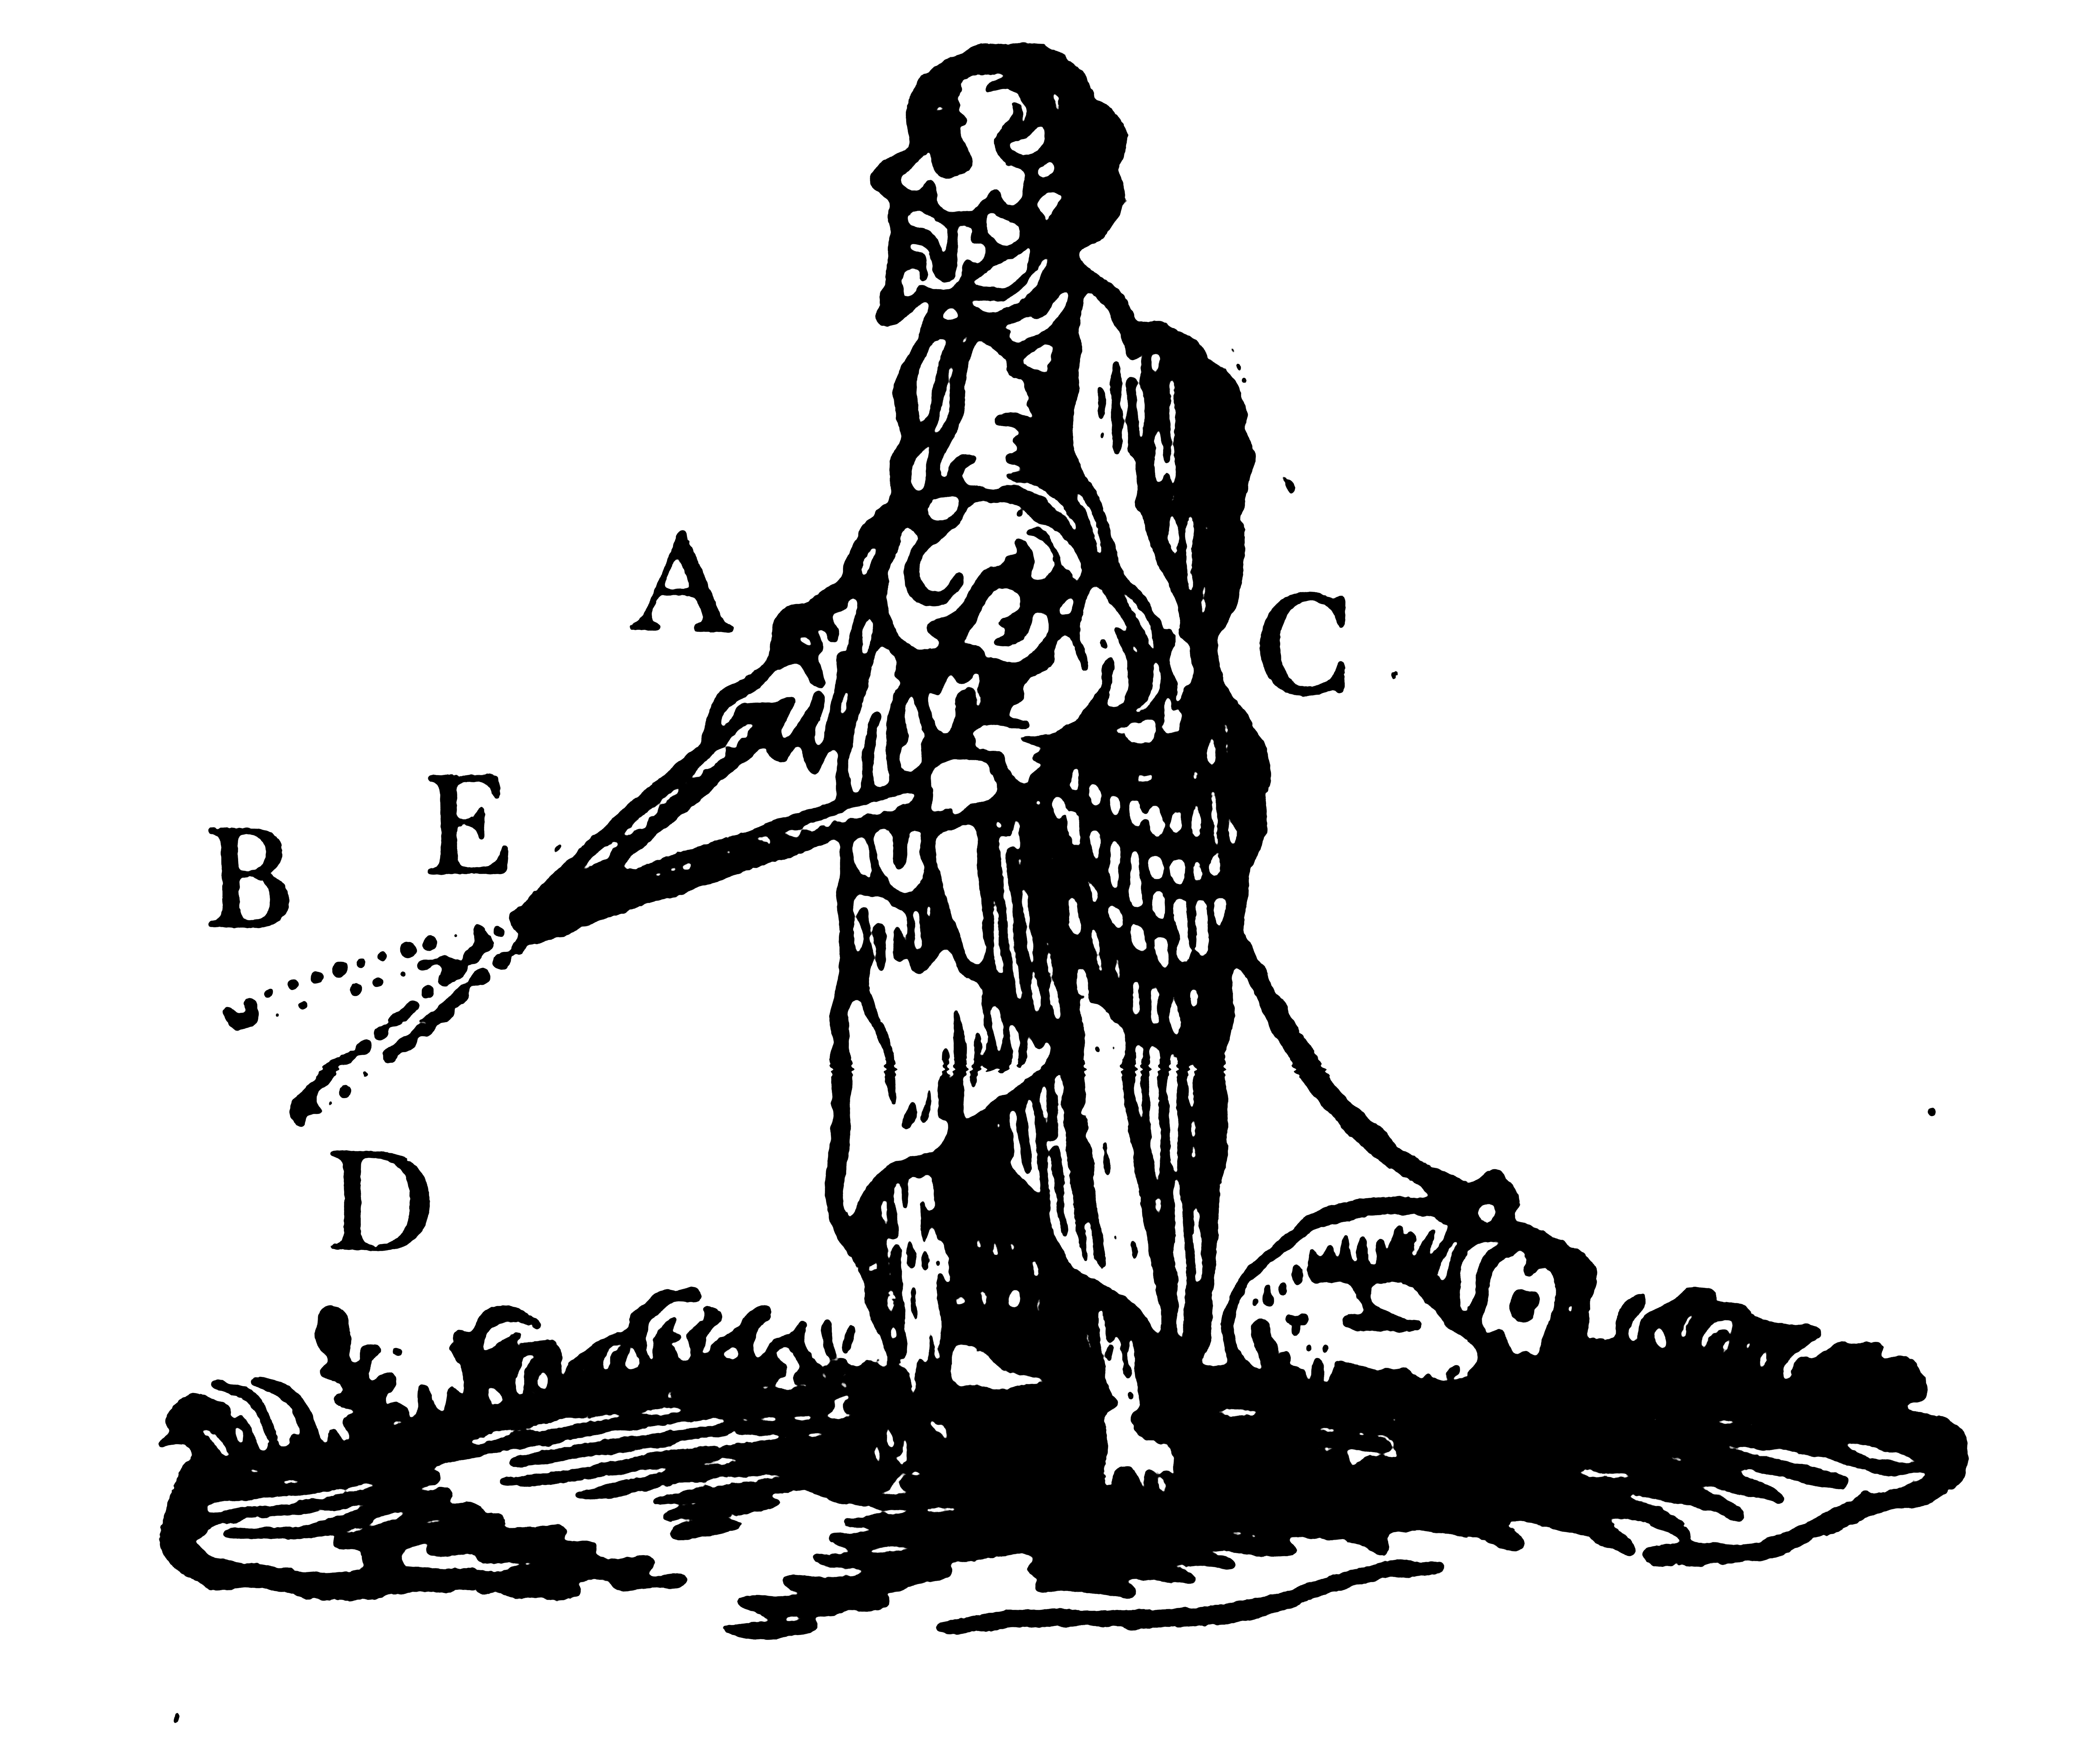
\includegraphics[scale=2]{graphics/blind.jpeg}
	\caption{\citealt{Descartes:1637uq}}
	\label{fig:blind}
\end{figure}

What is it about vision that constitutes the whole problem of vision as well as its peculiar virtue? Merleau-Ponty describes vision as a kind of action at a distance. This can suggest that the problem concerns the causal mechanisms that underly visual perception. Suppose vision is a kind of action at a distance. A problem would arise if one further held that causation, or at least immediate causation, requires contact. If causation requires contact, there is no action at a distance. This is misleading, however. Given the state of optical knowledge even at the time of Merleau-Ponty's writing, there was no serious question whether visual perception involved action at a distance in this sense. Light reflected, transmitted, and emitted from the scene travels to the perceiver and so irradiates their sensory surfaces, in Quine's \citeyearpar{Quine:1960rm} deflationary locution. 

In speaking of vision as a kind of action at a distance, Merleau-Ponty was not denying the existence of a proximal cause for vision, rather he was making a phenomenological observation, that vision presents us with objects located at a distance. That vision presents us with objects located at a distance, that vision is a mode of awareness of the distal environment, is plausibly that in which its peculiar virtue consists. Thus Aristotle claims that by means of vision animals capable of locomotion may move towards sources of vital nourishment just as they may flee mortal danger (\emph{De Anima} \textsc{iii} 12 434\( ^{a} \)81--82). Describing the ability to see objects located at a distance as the peculiar virtue of vision perhaps overstates the case. Audition is a distal sense as well. One may hear a distant predator just as one may see it. However, it remains easy to appreciate the utility of vision presenting objects located at a distance. 

The ubiquity which is the whole problem of vision concerns less the causal mechanisms that underly the presentation in vision of objects located at a distance than with the nature of their visual presentation. An Aristotelian might suggest, on Merleau-Ponty's behalf, that action in the slogan ``action at a distance'' refers less to the object of perception acting upon the perceiver, whether mediately or immediately, than to perceptual activity, understood as \emph{energeia}, the seeing of the object. Since the exercise of our visual capacity is the presentation in visual perception of the distal object, then action at a distance would instead refer to the visual presentation of an object located at a distance. Whether or not and to what extent Merleau-Ponty would have accepted the Aristotelian suggestion, the conclusion which we have reached by means of it, that the ubiquity which is the whole problem of vision concerns the visual presentation of objects located at a distance, is an understanding of that problem genuinely shared with Merleau-Ponty.

What is potentially problematic about the visual presentation of objects located at a distance? Given that the whole problem of vision concerns the presentation of objects located at a distance, somehow the distal character of the visible object must be inconsistent or at least in tension with the claim that it is presented in visual experience, on a compelling or at least plausible conception of visual presentation. The problem is usefully developed in terms of Broad's discussion of vision in ``Elementary reflections on sense perception''. There he writes:

% section a_puzzle_about_perception_at_a_distance (end)

\section{Empedocles and the answer in the style of Gorgias} % (fold)
\label{sec:empedocles_and_the_answer_in_the_style_of_gorgias}



% section empedocles_and_the_answer_in_the_style_of_gorgias (end)

\section{Transparency in \emph{De Anima}, a surprising definition} % (fold)
\label{sec:transparency_in_de anima_a_surprising_definition}



% section transparency_in_de anima_a_surprising_definition (end)

\section{Transparency in \emph{De Sensu}} % (fold)
\label{sec:transparency_in_de sensu}

% section transparency_in_de sensu (end)

% Bibligography
\bibliographystyle{plainnat} 
\bibliography{Philosophy} 

\end{document}
